\documentclass[a4paper, nofonts, nocap]{ctexart}

\usepackage[margin=1in]{geometry}
\usepackage[square, super]{natbib}
\usepackage{underscore}

\usepackage{fontspec}
\setmainfont{Arial}
\setsansfont{Arial}
\setmonofont{Consolas}

\usepackage{xeCJK}
\setCJKmainfont[BoldFont={FZDaHei-B02S}, ItalicFont={FZXingKai-S04S}]{FZLanTingHei-R-GBK}
\setCJKsansfont{FZLanTingHei-R-GBK}
\setCJKmonofont{FZLanTingHei-R-GBK}

\pagestyle{plain}

\title{点对点聊天软件 \\ \begin{large}——网络实验课期末PJ \end{large}}
\author{梁晓涛\quad 13307130319}
\date{\today}


\begin{document}

\maketitle

\section{开发环境}
只使用了python标准库的自带模块,理论上支持大部分Unix平台和Windows操作系统,但图形化界面的效果在不同操作系统会不同。
\begin{description}
	\item[操作系统] Ubuntu 14.04
	\item[编程语言] Python 3.4
		\begin{description}
			\item[网络] socket
			\item[图形化界面] tkinter
		\end{description}
\end{description}

\section{协议设计}
协议的消息格式分两种,一种用于发送聊天的内容,另一种用于回复聊天的内容是否发送成功。

发送聊天内容的消息的格式如图1所示。头部和发送的内容之间使用回车换行符"\textbackslash r\textbackslash n"分隔。头部是用空格分隔的3个字段,第一个字段是"SEND",表示该消息用于发送聊天内容,第二个字段表示发送的内容的长度,第三个字段是发送者的自己指定的用户名。可以注意到,用户名包含空格、发送的内容包含回车换行符,都不影响消息的解析,但用户名不允许包含回车换行符。

\begin{figure}[ht]
	\centering
	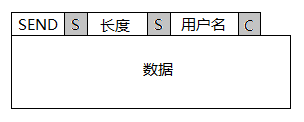
\includegraphics{images/send.png}
	\caption{发送聊天内容的报文的格式}
\end{figure}

回复发送状态的消息的格式如图2所示。同样地,头部和发送的内容之间使用回车换行符"\textbackslash r\textbackslash n"分隔,但发送的内容往往为空。头部是用空格分隔的3个字段,第一个字段是"RESPONSE",表示该消息用于回复发送状态,第二个字段表示消息的状态码,第三个字段表示状态码对应的原因短语。

\begin{figure}[ht]
	\centering
	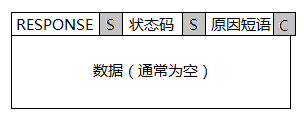
\includegraphics{images/response.png}
	\caption{响应报文的格式}
\end{figure}

\section{软件设计}
\begin{itemize}
	\item 采用P2P模型,每一方既是服务器也是客户端。
	\item 整个软件只由一个脚本文件组成,服务器和客户端分别属于不同的线程。
	\item 服务器线程对接收到的每一条消息进行解析,如果头部不规范,会向发送方回复出错的报告;如果头部规范,会向发送方回复发送成功的报告,并把信息的内容显示到聊天窗口中。
	\item 客服端线程会在每次用户点击发送按钮后,将文本框中的聊天文本封装并发送。如果发送失败,如网络不连通或消息格式不正确,状态栏会显示错误的原因;如果发送成功,状态栏会显示一条发送成功的语句,并将发送的聊天内容显示到聊天窗口中,同时清除文本框中的文本。
	\item 图形化界面包括从上到下的4个部分,依次是显示用户名及网络地址的区域,显示聊天内容的窗口,包含滚动条和发送按钮的文本编辑窗口,以及显示发送状态的状态栏。
\end{itemize}

\section{软件使用}
直接运行脚本,一开始需要在对话框内输入以下内容
\begin{enumerate}
	\setlength{\itemindent}{2em}
	\item 用户的自定义用户名
	\item 用于本地服务器的端口号
	\item 远程用户的IP地址
	\item 远程用户的端口号
\end{enumerate}

如图3所示是各个输入项的默认值。如果是两个软件运行在同一台电脑上,那么IP地址都填127.0.0.1,而两个端口号必须不一样。
\begin{figure}[ht]
	\centering
	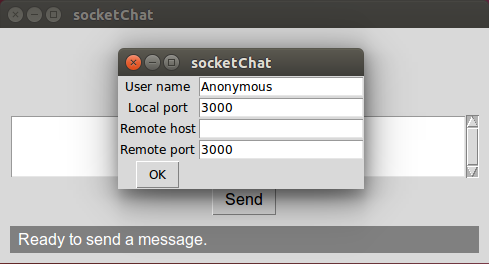
\includegraphics[scale=0.8]{images/dialog.png}
	\caption{对话框的默认值}
\end{figure}

一旦点击对话框后的按钮后,就可以开始聊天。刚开始的界面如图4所示,发送失败的界面如图5所示,发送成功的界面如图6所示。图6和图7是两个用户在同一时刻的软件界面。
\begin{figure}[ht]
	\centering
	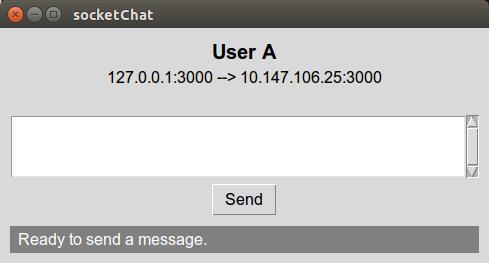
\includegraphics[scale=0.8]{images/init.png}
	\caption{初始界面}
\end{figure}
\begin{figure}[ht]
	\centering
	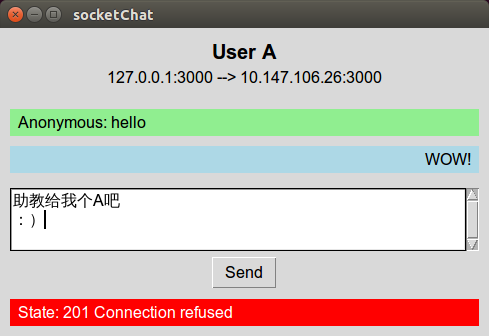
\includegraphics[scale=0.8]{images/fail.png}
	\caption{网络连接失败}
\end{figure}
\begin{figure}[ht]
	\centering
	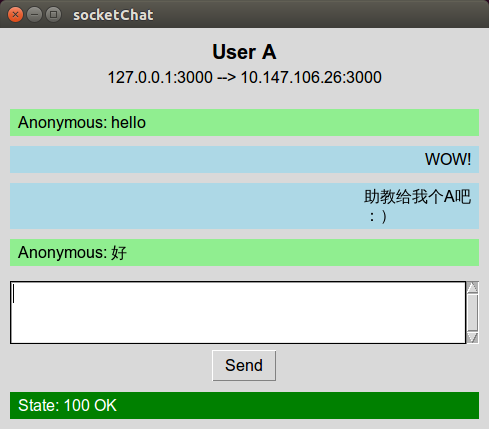
\includegraphics[scale=0.8]{images/success.png}
	\caption{发送成功}
\end{figure}
\begin{figure}[ht]
	\centering
	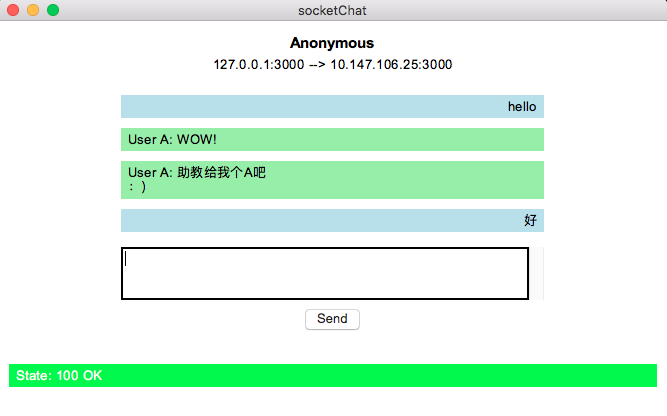
\includegraphics[scale=0.6]{images/two.png}
	\caption{另一个用户的界面}
\end{figure}

退出的时候需要先关闭聊天窗口,再用Ctrl+c关闭整个程序。
\end{document}


